\documentclass{beamer}
 
\usepackage[utf8]{inputenc} 
\usepackage[T1]{fontenc}
\usepackage{lmodern}
\usepackage{graphicx}
\usepackage[french]{babel}
 
\usetheme{Madrid}

\title[Présentation]{Soutenance du TPA}
\subtitle[\ldots]{Rapport}
\author[FTL]{Simon Bihel, Sebastien Gamblin, Josselin Gueneron, Julien Pezant, Paul Lemenager}
\institute[UCBN]{UCBN L2 Informatique Semestre 1}
\date{\today}
 
\begin{document}
\begin{frame}
	\maketitle
\end{frame}

\begin{frame}
	\frametitle{Plan}
	\tableofcontents
\end{frame}

\begin{frame}
	\frametitle{Présentation du jeu}
	\section{Présentation du jeu}
	
	\begin{figure}[H]
		\centering
		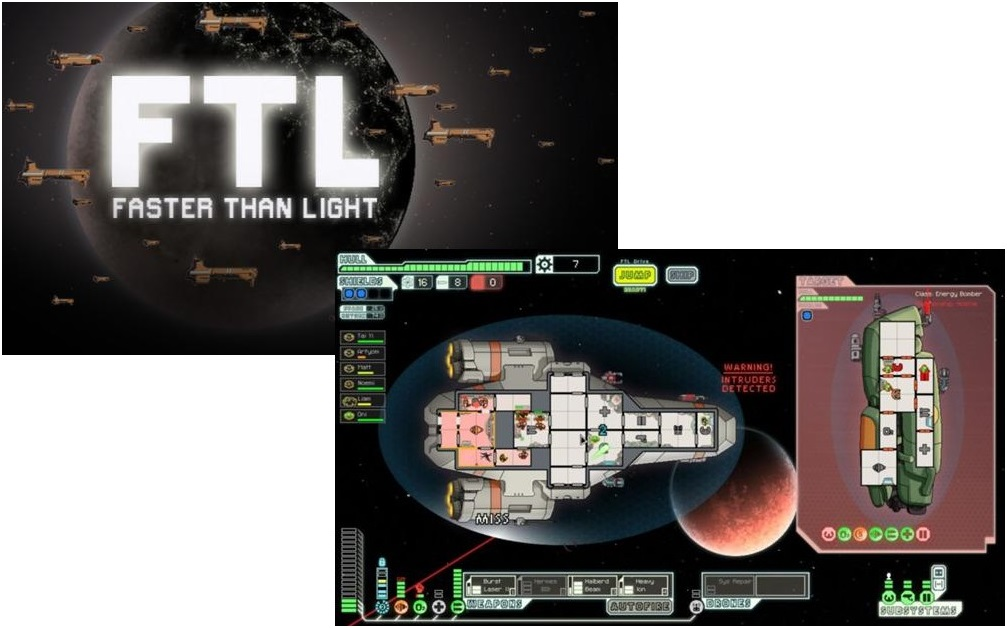
\includegraphics[width=0.7\linewidth]{ftl.jpg}
	\end{figure}
	
\end{frame}

\begin{frame}
	\frametitle{Présentation du projet}
	\section{Présentation du projet}
	
	Réalisation d'un programme permettant la modélisation de vaisseau FTL afin de les optimiser au mieux.
		
\end{frame}

\begin{frame}
	\frametitle{But du premier semestre}
	\section{But du premier semestre}
	Le but du premier semestre est de modéliser un générateur de combat le plus complet possible.
\end{frame}

\begin{frame}
	\frametitle{Les modules}
	\section{Les modules}
	
	\begin{figure}[H]
		\centering
		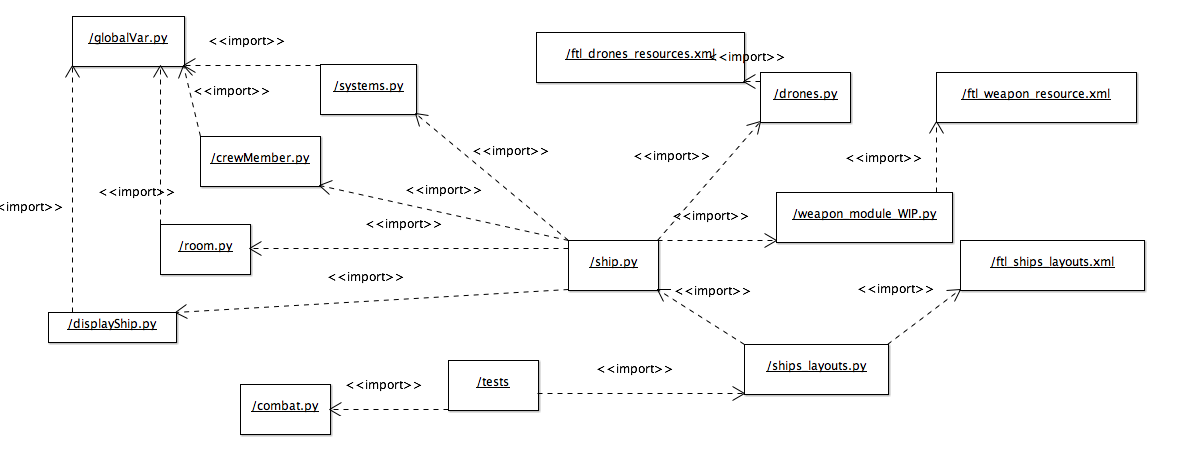
\includegraphics[width=1\linewidth]{smoothPackageDiagram.png}
	\end{figure}
	
\end{frame}

\begin{frame}
	\frametitle{Représentation d'un vaisseau}
	\section{Représentation d'un vaisseau}
	
	\begin{figure}[H]
		\centering
		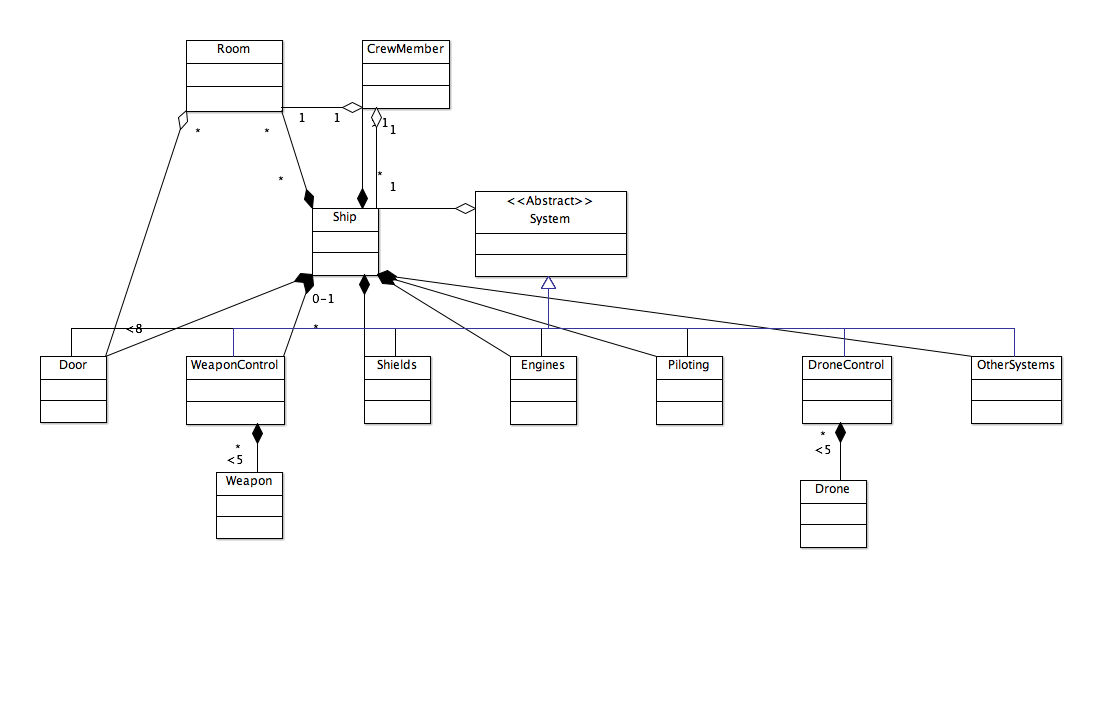
\includegraphics[width=1\linewidth]{smoothUmlDiagram.png}
	\end{figure}
\end{frame}

\begin{frame}
	\frametitle{Représentation d'un vaisseau}
	Les vaisseaux sont représentés aussi par le xml d'où sont extraites les informations des vaisseaux.
	
	\begin{figure}[H]
		\centering
		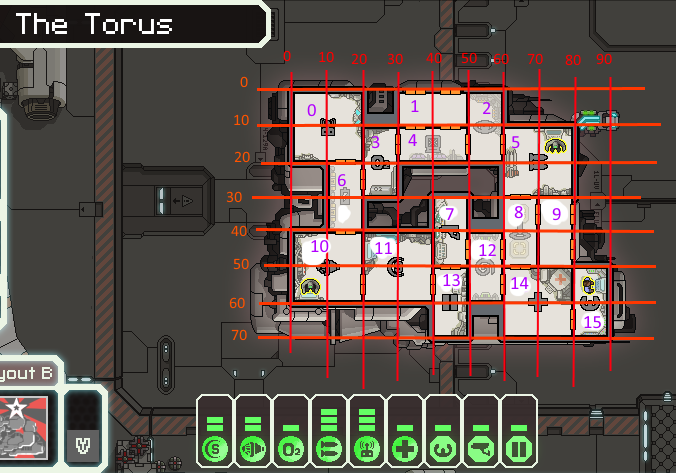
\includegraphics[width=0.7\linewidth]{engiCruiser_A_L.png}
	\end{figure}
	
\end{frame}

\begin{frame}
	\frametitle{Le combat}
	\section{Le combat}
	
	Décomposition d'un combat :
	\begin{itemize}
		\item Cooldowns
		\item Attaque
	\end{itemize}
	
\end{frame}

\begin{frame}
	\frametitle{Les cooldowns}
	\subsection{Les cooldowns}
	
	\begin{figure}[H]
		\centering
		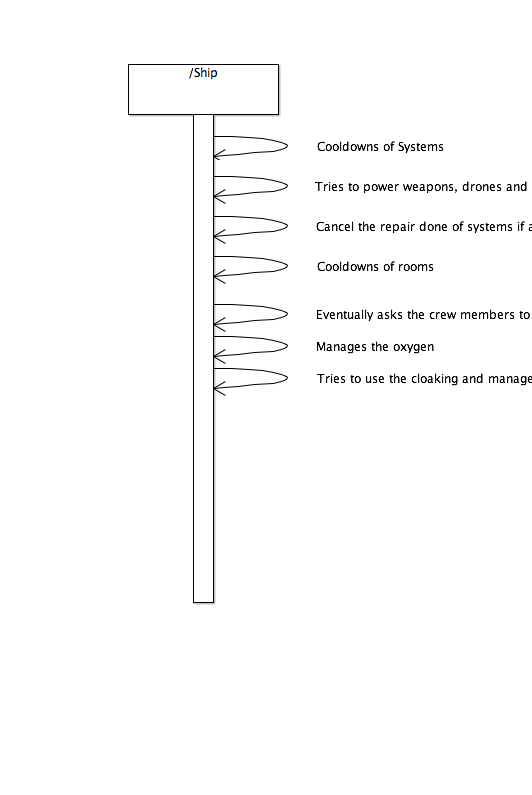
\includegraphics[width=0.75\linewidth]{smoothCooldownsDiagramShip}
	\end{figure}
	
\end{frame}

\begin{frame}
	\frametitle{L'attaque}
	\subsection{L'attaque}
	
	\begin{figure}[H]
		\centering
		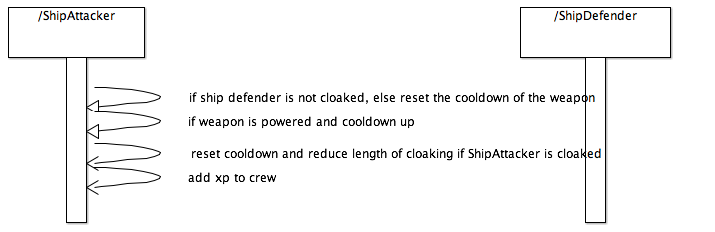
\includegraphics[width=0.75\linewidth]{smoothUseWeaponToAttackSequenceDiagramStart}
	\end{figure}
	
\end{frame}

\begin{frame}
	\frametitle{Un petit test}
	\section{Un petit test}
	
	Exemple de combat.
	
\end{frame}

\begin{frame}
	\frametitle{Conclusion}
	\section{Conclusion}
	
	Au cours du premier semestre, nous avons réussi à réaliser un moteur de combat qui, même s'il n'est pas complet, se rapproche du jeu original, ce qui nous permettra de finaliser notre projet : optimiser la recherche d'un vaisseau meilleur que les autres.
	
	Future pistes :
	\begin{itemize}
			\item Etablir arbitrairement des règles d'optimisation pour un vaisseau		
			\item Utiliser des systèmes experts afin de générer une intelligence artificielle qui pourra préférer tel équipement dans tel cas, optimiser l'utilisation des énergies des vaisseaux, ne pas avoir telle arme si elle est inutilisable, etc
			\item Utiliser un système d'algorithme génétique qui nous permettra de conserver les vaisseaux gagnants, et de les combiner pour qu'ils soient plus performants.
		\end{itemize}
	
\end{frame}


%\begin{frame}
%	\frametitle{les blocs}
%	\section{Test de bloc}
%	\begin{block}{Un bloc normal} % Bloc normal
%	A utiliser normalement, selon vos envies.
%	\end{block}
%	\begin{alertblock}{Bloc alerte} % Bloc alerte rouge
%	A utiliser pour alerter.
%	\end{alertblock}
%	\begin{exampleblock}{Un bloc exemple} % Bloc exemple vert
%	A utiliser pour donner un exemple.
%	\end{exampleblock}
%\end{frame}


 
\end{document}
